% https://es.overleaf.com/latex/templates/project-report/jpzczmpsdzwm

%%% Preamble
\documentclass[paper=leter, fontsize=11pt]{scrartcl}
\usepackage[utf8]{inputenc}
\usepackage[spanish,mexico]{babel}
\usepackage[T1]{fontenc}    % use 8-bit T1 fonts
\usepackage{lmodern}
\usepackage{hyperref}       % hyperlinks
\usepackage{lipsum}
\usepackage[square,numbers]{natbib}

\usepackage[protrusion=true,expansion=true]{microtype}	
\usepackage{amsmath,amsfonts,amsthm} % Math packages
\usepackage[pdftex]{graphicx}
\usepackage{url}

\usepackage{booktabs}

\usepackage{tikz}

\usepackage{caption}
\usepackage{subcaption}

\usepackage{listings}
\lstdefinestyle{mystyle}{
    basicstyle=\ttfamily\footnotesize,
    breakatwhitespace=false,         
    breaklines=true,                 
    captionpos=b,                    
    keepspaces=true,                 
    numbers=left,                    
    numbersep=5pt,                  
    showspaces=false,                
    showstringspaces=false,
    showtabs=false,                  
    tabsize=4
}

\lstset{style=mystyle}
\renewcommand{\lstlistingname}{Código}

\graphicspath{ {py/} }

\selectlanguage{spanish}
\usepackage[spanish,onelanguage,ruled]{algorithm2e}


%%% Custom sectioning
\usepackage{sectsty}
\allsectionsfont{\centering \normalfont\scshape}


%%% Custom headers/footers (fancyhdr package)
\usepackage{fancyhdr}
\pagestyle{fancyplain}
\fancyhead{}											% No page header
\fancyfoot[L]{}											% Empty 
\fancyfoot[C]{}											% Empty
\fancyfoot[R]{\thepage}									% Pagenumbering
\renewcommand{\headrulewidth}{0pt}			% Remove header underlines
\renewcommand{\footrulewidth}{0pt}				% Remove footer underlines
\setlength{\headheight}{13.6pt}


%%% Equation and float numbering
\numberwithin{equation}{section}		% Equationnumbering: section.eq#
\numberwithin{figure}{section}			% Figurenumbering: section.fig#
\numberwithin{table}{section}				% Tablenumbering: section.tab#


%%% Maketitle metadata
\newcommand{\horrule}[1]{\rule{\linewidth}{#1}} 	% Horizontal rule

%%% https://tex.stackexchange.com/a/118217
\usepackage{mathtools}
\DeclarePairedDelimiter\ceil{\lceil}{\rceil}
\DeclarePairedDelimiter\floor{\lfloor}{\rfloor}

\usepackage{amsmath}

\usepackage{tikz}

\title{
		%\vspace{-1in} 	
		\usefont{OT1}{bch}{b}{n}
		\normalfont \normalsize \textsc{Posgrado de Ingeniería de Sistemas} \\ [25pt]
		\horrule{0.5pt} \\[0.4cm]
		\huge Análisis de algoritmos de palíndromos \\
		\horrule{2pt} \\[0.5cm]
}
\author{
		\normalfont 								\normalsize
        Alberto Benavides\\[-3pt]		\normalsize
        \today
}
\date{}


%%% Begin document
\begin{document}
\maketitle

\section{Algoritmos de palíndromos} \nocite{aa}

Para esta tarea se desarrollan dos algoritmos de palíndromos en \texttt{Python}, uno iterativo y uno recursivo, presentes en los códigos \ref{iterativo} y \ref{recursivo}. Ambos reciben una cadena de texto, eliminan los espacios que contenga y retornan $\top$ en caso de tratarse de un palíndromo y $\bot$ de otra manera.

\begin{lstlisting}[caption={Algoritmo iterativo para encontrar palíndromos.}, captionpos=t, label={iterativo}]
def iterativo(s):
    s = s.replace(' ', '')
    mitad = int(len(s) / 2)
    if mitad == 0:
        return True
    for i in range(mitad):
        print(s[i] + s[-1 - i])
        if s[i] != s[-1 - i]:
            return False
    return True
\end{lstlisting} 

\begin{lstlisting}[caption={Algoritmo recursivo para encontrar palíndromos.}, captionpos=t, label={recursivo}]
def recursivo(s):
    s = s.replace(' ', '')
    mitad = int(len(s) / 2)
    if mitad == 0:
        return True
    if(s[0] != s[-1]):
        return False
    return recursivo(s[1:-1])
\end{lstlisting}

\section{Diseño de experimentos}

Con el fin de intuir las diferencias entre tiempos de cómputo, se realiza un experimento computacional en el que se generan $N = 6\,000$ palíndromos de longitudes de cadena $n = \{ 0, 2, 4, \ldots, 2N \}$ obtenidos a partir de concatenar a $n / 2$ caracteres tomados al azar del alfabeto \texttt{ascii} de la librería \texttt{string} \cite{string} con los mismos caracteres en orden reverso. Por cada palíndromo, se realizaron $r = 1\,000\,000$ repeticiones con la librería \texttt{timeti} \cite{timeit}. El tiempo que tomó completar estas $r$ repeticiones para cada cadena de longitud $n$ fue dividido entre $r$ para obtener el promedio de milisegundos de cada operación.

Los resultados de estos experimentos computacionales demuestran que el algoritmo iterativo toma más tiempo que el recursivo. Las diferencias en milisegundos entre los tiempos $t_i$ del algoritmo iterativo con respecto a los tiempos $t_r$ del algoritmo recursivo se muestran en la figura \ref{dif_i_r}. Muy pocos tiempos de cómputo del algoritmo recursivo son superiores a los del algoritmo iterativo para la misma cadena de texto, sin embargo esto puede deberse a los distintos procesos que se ejecutan por el sistema operativo donde se realizaron estos experimentos. Una discusión al respecto puede leerse en \url{https://stackoverflow.com/q/52251680}.

\begin{figure}
    \centering
    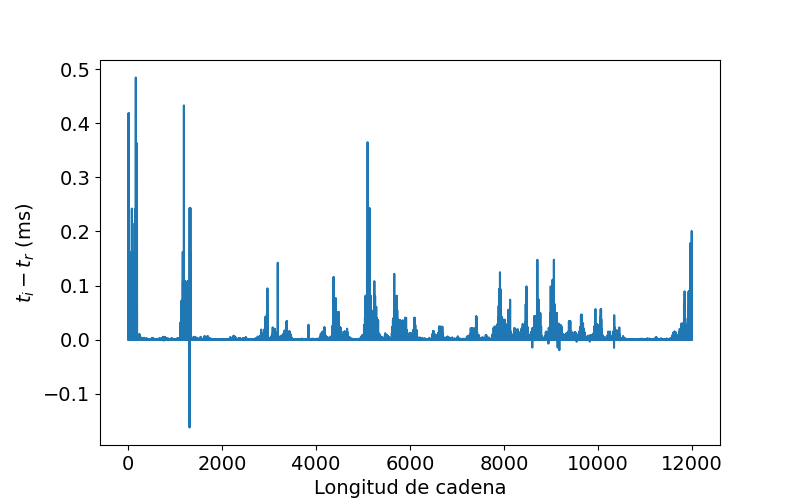
\includegraphics[width=0.8\textwidth]{dif_i_r.png}
    \caption{Diferencias en milisegundos entre los tiempos de cómputo del algoritmo iterativo ($t_i$) y los del recursivo ($t_r$).}
    \label{dif_i_r}
\end{figure}

\section{Análisis de los algoritmos}

El análisis de los algoritmos se realiza siguiendo los ejemplos del material de curso compartido por \citeauthor{aa} \cite{aa} en sus notas de curso.

\subsection{Algoritmo iterativo}
Aquí, se tiene una cadena $s$ de entrada, de longitud $l$, compuesta por $l$ caracteres hubicados en una posición $s_i, i \in \{0, 1, 2, \ldots, l\}$. La complejidad computacional de este algoritmo viene dada por
\begin{itemize}
    \item $f_0$: Lectura de la cadena $s$, $\mathcal{O}(1)$;
    \item $f_1$: Obtención de la longitud $l$ de $s$, $\mathcal{O}(1)$;
    \item $f_2$: Asignación de $m = \floor*{l / 2}$ como mitad de la longitud de $s$, $\mathcal{O}(1)$;
    \item $f_3$: Condición que evalúa $m = 0$,  con $\mathcal{O}(1)$;
    \item $f_4$: Condición que evalúa $s_i = s_{l - 1 - i}$, $\mathcal{O}(1)$;
    \item $f_5$: Ciclo que itera sobre $i \in \{0, 1, 2, \ldots, m\}$, $\mathcal{O}(m + f_4)$;
\end{itemize}
de donde se tiene que la complejidad computacional de este algoritmo es
\begin{equation}
    \mathcal{O}(f_0 + f_1 + f_2 + f_3 + f_5) = \mathcal{O}(4 + n / 2).
\end{equation}

\subsection{Algoritmo recursivo}

La función $R$ para el algoritmo recursivo de detección de palíndromos recibe también una cadena de caracteres $s$ de longitud $l$ de caracteres con $c_i$ con posiciones $i \in \{0, 1, 2, \ldots, l - 1\}$ cuya función es
\begin{equation}
    R(s) = \left\{\begin{matrix}
       \top & \floor*{l /2} = 0\\ 
       \bot & c_0 \neq c_{l - 1}\\
       R(s(0, l-1)) & \floor*{l /2} \neq 0 \land c_0 = c_{l - 1}
       \end{matrix}\right.
\end{equation}

Esta función puede simplificarse en la función modificada $R^*$ que toma como parámetro inicial $l$
\begin{equation}
    R^*(n) = \left\{\begin{matrix}
        1 & n \leq 1\\ 
        R^*(n - 2) & n > 1
        \end{matrix}\right.
\end{equation}
de donde obtenemos
\begin{equation}
    \begin{split}
    R^* & = R^*(n - 2) \\ 
    & = R^*((n - 2) - 2) \\
    & = R^*(((n - 2) - 2) - 2) \\
    & = \ldots
    \end{split}
\end{equation}
y por expansión
\begin{equation}
    \begin{split}
    R^*(n) & = R^*(n - 2) \\
    R^*(n - 2) & = R^*((n - 2) - 2) = R^*(n - 4)\\
    R^*(n - 4) & = R^*(((n - 2) - 2) - 2) = R^*(n - 6) \\
    \ldots \\
    R^*(n - 2i) & = R^*((n - 2i) - 2) \\
    \ldots \\
    R^*(n - 2 \cdot \floor*{n / 2}) & = \left\{\begin{matrix}
        R^*(1) \\ 
        R^*(0)
        \end{matrix}\right.
    \end{split}
\end{equation}
o sea
\begin{equation}
\begin{split}
    R^*(n) & = R^*(1) + \floor*{n / 2}\\
\end{split}
\end{equation}
lo que deja $\mathcal{O}(1 + \floor*{n / 2})$.

\bibliographystyle{plainnat}
\bibliography{Biblio}

\end{document}